\subsection{Messages and transactions}

As we said in \autoref{sec:accounts}, contracts can send messages or
transactions to other contracts in response to an event.

A transaction is a
single instruction constructed by an actor externally to the scope of Ethereum
\cite{wood2018ethereum}, it is serialized and included in the blockchain. It can
be used to transfer ether\footnote{The currency used within Ethereum} or to
trigger contract code.

A message is a virtual object that is not serialized and
exists only in the Ethereum execution environment.

\begin{figure}[h]
  \centering
  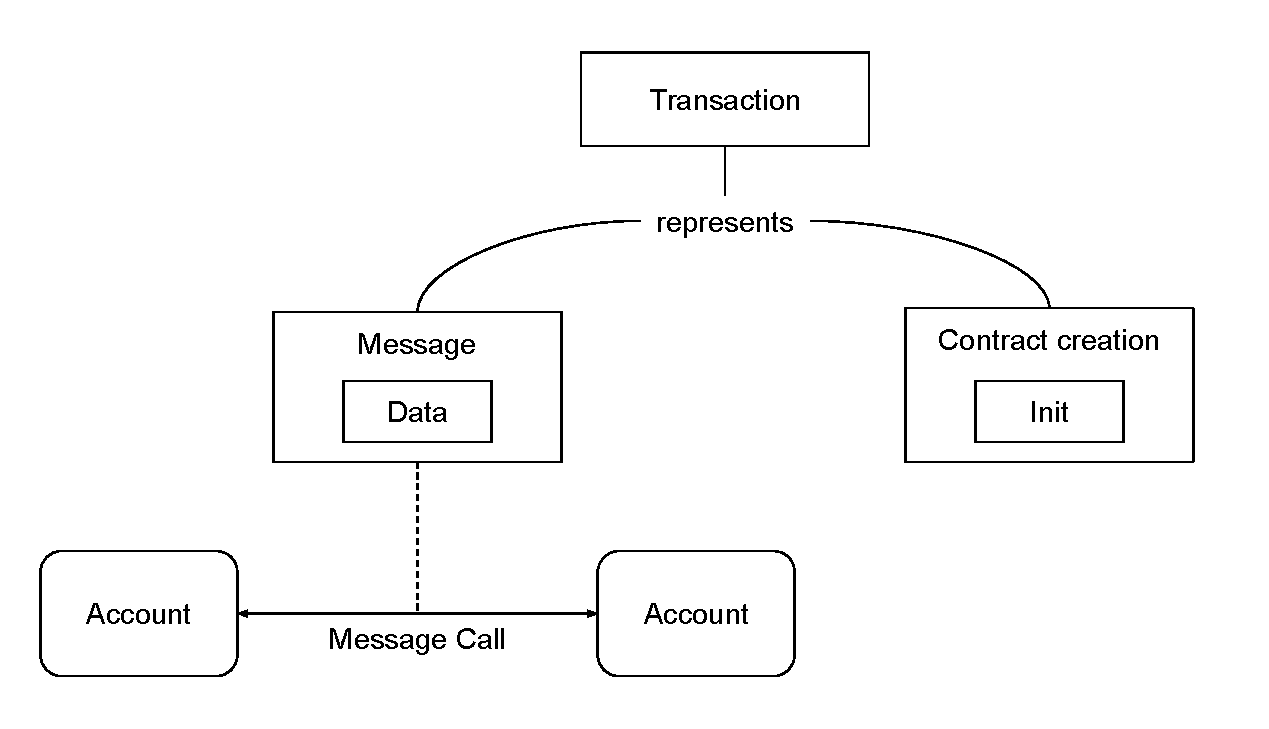
\includegraphics[width=\textwidth]{./res/img/messages-transactions.pdf}
\caption{Representation of the relation between message and transaction.}
\label{fig:messages-transactions}
\end{figure}